\documentclass{article}
\addtolength{\oddsidemargin}{-.875in}
\addtolength{\evensidemargin}{-.875in}
\addtolength{\textwidth}{1.0in}
\addtolength{\topmargin}{-0.5in}
\addtolength{\textheight}{1.00in}
\usepackage{wrapfig}
\usepackage{sidecap}
\usepackage{hyperref}
\usepackage[pdftex]{graphicx}
\usepackage[utf8]{inputenc}
\usepackage[spanish]{babel}

\title{Reporte de Actividades - Enero 2015 - Febrero 2018}
\author{Jaime E. Forero Romero\\Profesor Asociado - Departamento de
  F\'isica\\Universidad de los Andes}  
\begin{document}

\maketitle
\tableofcontents
\newpage

\section{Docencia}

\subsection{Cursos dictados}
\begin{tabular}{p{6.5cm} l c c}\hline
Curso & Semestre & Inscritos & Calificaci\'on (sobre
4.0)\\\hline
STAI & 2017-20 & - & -\\\hline
F\'isica II & 2017-10 & 68 & 3.43\\
M\'etodos Computacionales Avanzados & 2017-10 & 17 & 3.72\\ 
Taller de Astronom\'ia & 2017-10 & 19 & 4.00\\\hline
Astronom\'ia Popular (CBU) & 2016-10 & 92 & 3.78\\
M\'etodos Computacionales & 2016-20 & 20 & 3.77\\
Taller de Astronom\'ia & 2016-20 & 14 & 3.95\\\hline
F\'isica I & 2016-10 & 80 & 3.68\\
M\'etodos Computacionales Avanzados & 2016-10 & 9 & 3.83\\
Taller de Astronom\'ia & 2016-10 & 6 & 3.75\\\hline
Astronom\'ia Popular (CBU) & 2015-20 & 91 & 3.75\\ 
M\'etodos Computacionales & 2015-20 & 10 & 3.47\\
Taller de Astronom\'ia & 2015-20 & 70 & 3.92\\\hline
F\'isica I & 2015-10 & 96 & 3.86\\
Electromagnetismo II & 2015-10 & 6 & 3.65 \\
Taller de Astronom\'ia & 2015-10 & 10 & 3.86\\\hline
Total Estudiantes / Promedio Ponderado & & 608 & 3.75$\pm$0.14 \\\hline
\end{tabular}

\subsection{Desarrollo de nuevos cursos}
\begin{itemize}
\item Construcci\'on de un nuevo CBU: \emph{Astronom\'ia Popular}.
\item Construcci\'on de un nuevo curso para pregrado avanzado y
  posgrado: \emph{M\'etodos Computacionales Avanzados}.
\item Re-estructuraci\'on del curso Herramientas Computacionales en
  una metodolog\'ia \emph{flipped-classroom}.
\end{itemize}

\subsection{Educaci\'on Continuada}
\begin{itemize}
\item Abril 2017. Una adaptaci\'on del curso Herramientas Computacionales fu\'e
  dictada como un curso abierto y gratuito para estudiantes de
  Uniandes y otras universidades. El evento se llam\'o Python Bootcamp
  y se dict\'o en 16 horas de clase en dos d\'ias. El curso cont\'o
  con 100 asistentes. %\url{https://pythonbootcampuniandes.github.io/}
\item Agosto 2017. Una adaptaci\'on del CBU Astronom\'ia Popular se dict\'o como
  curso de 16 horas a trav\'es de Educaci\'on Continuada de
  Uniandes. El curso cont\'o con 8 asistentes.
\end{itemize}



\subsection{Tesis Dirigidas}

\begin{itemize}
\item 
\end{itemize}

\section{Investigaci\'on}


\subsection{Refereed Papers}

\begin{itemize}

\item[8]{\it Modelling the gas kinematics of an atypical Lyman alpha
emitting compact dwarf galaxy}, {\bf J. E. Forero-Romero}, M. Gronke, M. C. Remolina-Guti\'errez,
Nicol\'as Garavito-Camargo, Mark Dijkstra, MNRAS submitted. 

\item[7]{\it Tracing the cosmic web}, N. I. Libeskind, R. van de Weygaert, M. Cautun, B. Falck, E.
Tempel, T. Abel, M. Alpaslan, M. A. Aragón-Calvo, {\bf
  J. E. Forero-Romero},  R. Gonzalez, S. Gottl\"ober, O. Hahn 13 ,
W. A. Hellwing, Y. Hoffman, B. J. T. Jones, F. Kitaura, A. Knebe,
S. Manti, M. Neyrinck, S. E. Nuza, N. Padilla, E. Platen,
N. Ramachandra, A. Robotham, E. Saar, S. Shandarin, M. Steinmetz,
R. S. Stoica, Th. Sousbie, G. Yepes, MNRAS accepted.  

\item[6]{\it Boosting Lya and HeII 1640A Line Fluxes from Pop III
  Galaxies: Stochastic IMF Sampling and Departures from
  Case-B}. L. Mas-Ribis, M. Dijkstra, {\bf J.E. Forero-Romero},
  ApJ, 833, 1, 2016.

\item[5]{\it Quantifying and controlling biases in dark matter halo
  concentration estimates}, C.N. Poveda-Ruiz, {\bf
  J.E. Forero-Romero}, J.C. Mu\~noz-Cuartas, ApJ, 832, 2, 2016. 

\item[4]{\it Impact of Cosmic Variance on the Galaxy-Halo Connection
  for Lyman-$\alpha$ emitters}.  J.E. Mej\'ia-Restrepo, {\bf
  J.E. Forero-Romero}, ApJ, 821, 1, 2016

\item[3]{\it SPOKES: An end-to-end simulation facility for
  spectroscopic cosmological surveys}, 
	Nord, B.; Amara, A.; R\'efr\'egier, A.; Gamper, La.; Gamper, Lu.;
        Hambrecht, B.; Chang, C.; {\bf Forero-Romero, J. E.}; Serrano, S.;
        Cunha, C.; Coles, O.; Nicola, A.; Busha, M.; Bauer, A.;
        Saunders, W.; Jouvel, S.; Kirk, D.; Wechsler, R., Astronomy
        and Computing, 15, 1, 2016
\item[2]{\it The Local Group in the Cosmic Web}, 	
Forero-Romero, J. E.; González, R., The Astrophysical Journal, Volume
799, Issue 1, article id. 45, 6 pp. (2015). 
\item[1] {\it Tensor anisotropy as a tracer of cosmic voids}, 
Bustamante, Sebastian; Forero-Romero, Jaime E., Monthly Notices of the
Royal Astronomical Society, Volume 453, Issue 1, 2015.
\end{itemize}

\subsection{Non-Refereed Papers}

\begin{itemize}
\item[2]
\end{itemize}


\subsection{Conference Proceedings}

\begin{itemize}
\item {\it The influence of environment on the HI mass functions in cosmological simulations}, 
J. D. Prada-Gonzalez, M. G. Jones, J. E. Forero-Romero, M. P. Haynes, Revista Mexicana de Astronomía y Astrofísica, 132, 49, 2017.
\end{itemize}

\subsection{Asesor\'ia de postdocs}

\begin{itemize}
\item Ver\'onica Arias. 2015-2016.

\end{itemize}

\subsection{Evaluador Externo}
\begin{itemize}
\item Universidad de Antioquia (Colombia).
\item MNRAS (Reino Unido).
\item Fondecyt (Chile).
\end{itemize}

\subsection{Funding}
\begin{tabular}{l l l p{2.4cm} p{4.0cm} c}\hline
N$^{o}$ & Fecha & Duraci\'on & Instituci\'on & Proyecto & Monto \\\hline
1 & 1.10.2016 & 36 meses & COLCIENCIAS & Simulaciones y Observaciones del Universo a Gran Escala & 200 Millones COP\\\hline
2 & 1.03.2017 & 48 meses & Uni\'on Europea & Latin-American Galaxy Formation Network & 1.4 Millones EURO \\\hline
3 & 1.10.2017 & 24 meses & Uniandes & Machine Learning aplicado a b\'usqueda de transientes astronom\'omicos& 120 Millones COP \\
\\\hline 
\end{tabular}

\subsection{Visitas de investigaci\'on}

\begin{tabular}{l l l p{3.5cm} p{5.0cm}}\hline
N$^{o}$ & Fecha & Duraci\'on & Instituci\'on & Proyecto \\\hline
2 & 12-07-2015 & 2 semanas & Durham University & Colaboraci\'on DESI\\
1 & 22-09-2014 & 1 semana & Lawrence Berkeley National
Laboratory & Colaboraci\'on DESI\\\hline
\end{tabular}

\subsection{Presentaciones t\'ecnicas}

\begin{tabular}{l c l l p{2cm} p{5cm}}\hline
N$^{o}$ & Fecha & Pa\'is & Ciudad & Lugar & T\'itulo \\\hline
5 & 12-12-2014 & Ecuador & Quito & Universidad San Francisco de Quito & Galaxias y Cosmolog\'ia\\
4 & 2-12-2014 & Colombia & Pasto & Congreso Colombiano de Astronom\'ia y Astrof\'isica & Cosmolog\'ia y formaci\'on de estructuras: una perspectiva computacional\\
3 & 4-11-2014 & Korea & Seoul & 6th KIAS Workshop on Cosmology and Structure Formation & The Place of The local group in the cosmic Web\\
2 & 17-10-2014 & Colombia & Bogot\'a & Universidad de los Andes & The
Place of the Local Group in the Cosmic Web\\
1 & 26-08-2014 & Germany & Potsdam & 11th Potsdam Thinkshop & The Local
Group in the Cosmic Web\\ \hline
\end{tabular}


\begin{figure}[!h]
\begin{center}
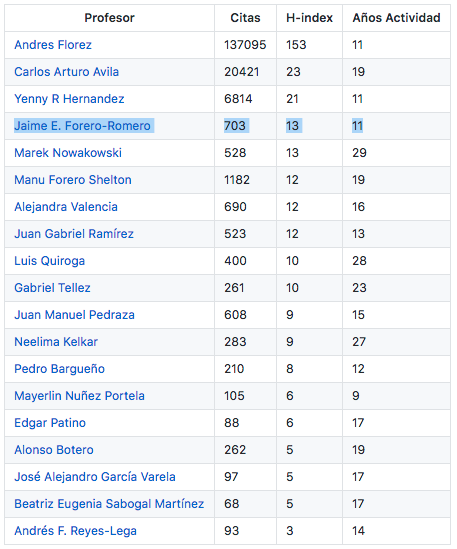
\includegraphics[scale=0.50]{scholar_fisica.png}
\caption{Figura para el problema 1. \url{https://github.com/forero/gsc/blob/master/info/fisica_uniandes.md}\label{table:fisica}}
\end{center}
\end{figure}


\begin{figure}[!h]
\begin{center}
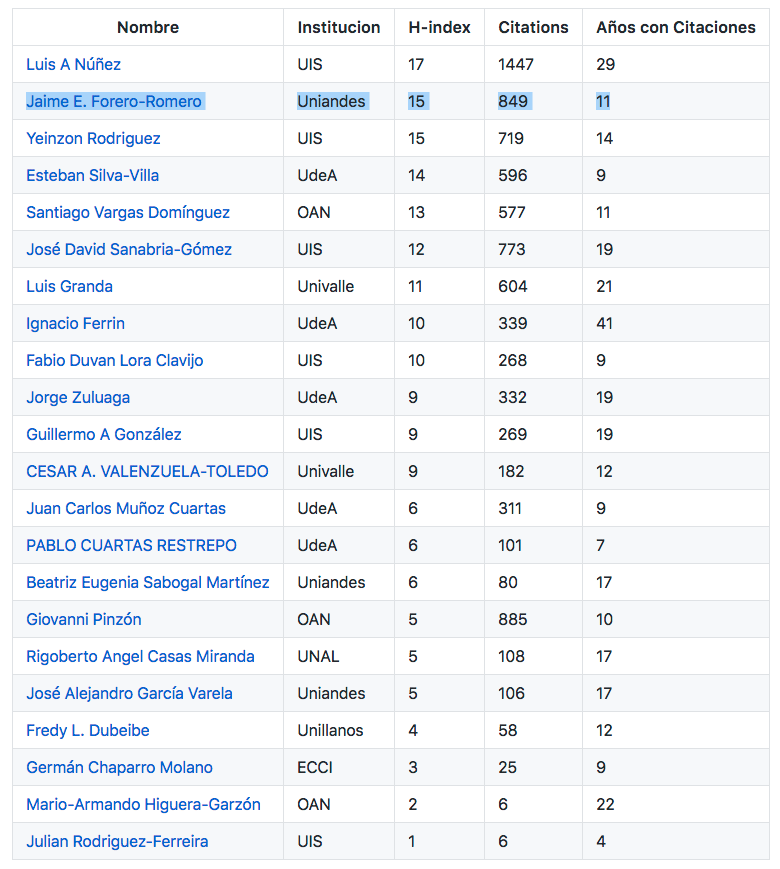
\includegraphics[scale=0.60]{scholar_astronomia.png}
\caption{Figura para el problema 1. \url{https://github.com/forero/gsc/blob/master/info/fisica_uniandes.md}\label{table:astro}}
\end{center}
\end{figure}

\newpage

\section{Desarrollo Institucional}



\subsection{Comit\'es}
\begin{itemize}
\item {Representante del Departamento de F\'isica en el comit\'e
  de c\'omputo de alto rendimiento de la facultad de ciencias en 2015-10}.
\item {}
\end{itemize}


\subsection{Visibilidad nacional e internacional}
\begin{itemize}
\item {Organizador de la una escuela Andina de Cosmolog\'ia (1 mes de
  duraci\'on, 4 instructores internacionales, 20 estudiantes de la
  regi\'on andina), Junio2015.}
\item {Co-organizador del segundo workshop Astronom\'ia en los Andes
  (cerca de 100 asistentes), Julio 2015.}
\item {Co-editor de las memorias del segundo workshop Astronom\'ia en
  los Andes, Julio 2015.}
\item {Lidero la Oficina Regional de Astronom\'ia para el
  Desarrollo. Esta Oficina es una red colaboraci\'on entre Colombia,
  Venezuela, Ecuador, Per\'u y Chile con el patrocinio de la Uni\'on
  Astron\'omica Internacional. La creaci\'on de la red se formaliz\'o
  en Julio del 2015 en la Universidad de los Andes.}   
\end{itemize}

\subsection{Presentaciones p\'ublicas}

\begin{tabular}{l l l l p{3cm} p{4cm}}\hline
N$^{o}$ & Fecha & Pa\'is & Ciudad & Lugar & T\'itulo\\\hline
3 & 21-05-2015 & Colombia & Bogot\'a & Conversatorio Maloka & De d\'onde vengo yo. Luz, estrellas y galaxias.\\
2 & 11-03-2015 & Colombia & B/manga & Caf\'e Cient\'ifico & Cielos Fluidos y Astronom\'ia Perif\'erica. Dos proyectos de Arte y Astronom\'ia.\\
1 & 20-09-2014 & Colombia & Bogot\'a & Seminario de Estudiantes del
Planetario de Bogot\'a& Una carrera astron\'omica \\\hline
\end{tabular}



\end{document}
